\documentclass[slidestop,compress,mathserif]{beamer}
%\documentclass[slidestop,compress,mathserif,handout]{beamer}

%\documentclass[xcolor=dvipsnames,handout]{beamer}
%\documentclass[xcolor=dvipsnames]{beamer}

%\documentclass[handout]{beamer}

%%% To get rid of solutions on handouts:
\newcommand{\soln}[1]{\textit{\textcolor{darkGray}{#1}}}				% For slides
%\newcommand{\soln}[1]{ }	% For handouts

% to get pausing to work properly on slides
\newcommand{\hide}[1]{#1}	% For slides
%\newcommand{\hide}[1]{ }	% For handouts


%\usepackage{multicol}
\usepackage{amsfonts}
%\usepackage[pdftex,dvipsnames]{color}
\usepackage{graphicx}
\usepackage{subfigure}
%\usepackage{picinpar}
\usepackage{pifont}
\usepackage{pgf,pgfarrows,pgfnodes}
%\usepackage{wasysym,manfnt,phaistos,empheq}
\usepackage[english]{babel}
\usepackage{pgfpages}
\usepackage{natbib}
\usepackage{hyperref}
\usepackage{multimedia}
%\usepackage{amsfonts,amstext,amssymb,amsbsy,amsopn,amsthm,eucal,latexsym,mathrsfs}
\usepackage{amsmath,amsfonts,amstext,amssymb,amsbsy,amsopn,amsthm,eucal,latexsym,mathrsfs}
\usepackage{ulem}
\usepackage{setspace}
\usepackage{array}
%\usepackage{rotating}
\usepackage{multirow}
\usepackage{verbatim}
\usepackage{multicol}

\setbeamertemplate{navigation symbols}{}

%\usepackage{tikz}
%\usetikzlibrary{arrows,shapes,trees,backgrounds}


%\setbeameroption{show notes on second screen}
%\setbeameroption{show notes}
%\setbeameroption{show only notes}

\definecolor{links}{HTML}{2A1B81}
\hypersetup{colorlinks,linkcolor=,urlcolor=links}

\newtheorem*{principle}{Inscrutibility Principle}
\newtheorem*{punchline}{Punch Line}
\newtheorem{defn}{Definition}

\definecolor{Scarlet}{RGB}{140,17,17}
\definecolor{VassarRed}{RGB}{128,0,0}

% "dinglist" environment
  \renewenvironment{dinglist}[2][blue]
  {\begin{list}{\textcolor{blue}{\ding{#2}}}{}}{\end{list}}
  % Symbol definitions for these lists
  \newcommand{\DingListSymbolA}{43}
  \newcommand{\DingListSymbolB}{243}
  \newcommand{\DingListSymbolC}{224}
  \newcommand{\DingListSymbolD}{219}
  \newcommand{\DingListSymbolCheck}{52}
  \newcommand{\DingListSymbolCross}{56}


  \newenvironment{ballotenv}
{\only{%
\setbeamertemplate{itemize item}{\ding{45}}%
\setbeamertemplate{itemize subitem}{\ding{46}}%
\setbeamertemplate{itemize subsubitem}{\ding{46}}}} {}
\setbeamertemplate{itemize item}{\ding{49}}
\setbeamertemplate{itemize subitem}{\ding{47}}
\setbeamertemplate{itemize subsubitem}{\ding{47}}


%User defined colors: See colors section
\xdefinecolor{oiBlue}{rgb}{0.15, 0.35, 0.55}
\xdefinecolor{gray}{rgb}{0.5, 0.5, 0.5}
\xdefinecolor{darkGray}{rgb}{0.3, 0.3, 0.3}
\xdefinecolor{darkerGray}{rgb}{0.2, 0.2, 0.2}
\xdefinecolor{rubineRed}{rgb}{0.89,0,0.30}
\xdefinecolor{linkCol}{rgb}{0.11,0.49,0.95}	
\xdefinecolor{irishGreen}{rgb}{0,0.60,0}	
\xdefinecolor{darkturquoise}{rgb}{0.44, 0.58, 0.86}
\definecolor{lightGreen}{rgb}{0.533,0.765,0.42}
\xdefinecolor{Regalia}{HTML}{522D80}
\xdefinecolor{ClemsonOrange}{HTML}{EA6A20}

\definecolor{duke@LightGrey}{RGB}{200,200,200}\definecolor{DarkGreen}{RGB}{0,100,0}
\definecolor{Oranges}{RGB}{255,127,0}
\definecolor{LightGray}{RGB}{211,211,211}

%\setbeamertemplate{footline}{%
%  \raisebox{5pt}{\makebox[\paperwidth]{\hfill\makebox[10pt]{\scriptsize\insertframenumber}}}}

\setbeamercolor{equation background}{fg=black,bg=duke@LightGrey}
  % Boxed equation
  \newcommand{\eqbox}[2][0.6]{%
  \centerline{
  \begin{beamerboxesrounded}[lower=equation background,width=#1\hsize,shadow=true]{}
\parbox{#1\hsize}{%
      \[
        \textcolor{black} {#2}
      \]}
  \end{beamerboxesrounded}
}}

\AtBeginSection[] {
  \begin{frame}<beamer>\frametitle{Outline}
    \tableofcontents[currentsection,hideothersubsections]
  \end{frame}
}
%
%
%\AtBeginSubsection[] {
%  \begin{frame}<beamer>\frametitle{Outline}
%    \tableofcontents%[currentsection,currentsubsection]
%  \end{frame}
%}

%\usecolortheme[RGB={82,45,128}]{structure}
%\usecolortheme[RGB={162,80,22}]{structure}
\usecolortheme[RGB={128,0,0}]{structure}
\usetheme[secheader]{Boadilla}
%\usetheme[height=7mm]{Rochester}
%\usetheme{Copenhagen}
%\usetheme{Antibes}
%\usecolortheme{seahorse}
%\usecolortheme{crane}
%\usecolortheme{rose}
%\usefonttheme[onlylarge]{structurebold}
%\usefonttheme[onlymath]{serif}



\def\diag{{\rm diag}}


\def\E{\mathbb{E}}
\def\Prob{\mathbb{P}}
\def\argmin{{\rm argmin}}
\def\argmax{{\rm argmax}}
\def\Def{\stackrel{def}{=}}


\newtheorem{assumption}{Assumptions}
\newtheorem*{proposition}{Proposition}
\newtheorem*{remark}{Remark}



%\setbeamercolor{disc title}{bg=oiBlue!40!white!60,fg=blue}
\setbeamercolor{disc body}{bg= Regalia!20!white!80,fg= Regalia!80!black!90}

\setbeamercolor{clicker ungraded title}{bg=irishGreen!80!white!50,fg=irishGreen!30!black!90}
\setbeamercolor{clicker ungraded body}{bg=irishGreen!20!white!80,fg=irishGreen!30!black!90}

\setbeamercolor{clicker review title}{bg=gray!80!white!80,fg=oiBlue!80!black!90}
\setbeamercolor{clicker review body}{bg=gray!30!white!90,fg=oiBlue!80!black!90}

\setbeamercolor{code body}{bg=gray!20!white!80,fg=black}


% Custom commands
\newcommand{\degree}{\ensuremath{^\circ}}
\newcommand{\Note}[1]{
\rule{2.5cm}{0.25pt} \\ \textit{\scriptsize {\textcolor{rubineRed}{Note:} \textcolor{gray}{#1}}}}
\newcommand{\ct}[1]{
\vfill
{\tiny #1}}
\newcommand{\Remember}[1]{\textit{\scriptsize{\textcolor{orange}{Remember:} \textcolor{gray}{#1}}}}
\newcommand{\red}[1]{\textit{\textcolor{rubineRed}{#1}}}
\newcommand{\pink}[1]{\textit{\textcolor{rubineRed!90!white!50}{#1}}}
\newcommand{\green}[1]{\textit{\textcolor{irishGreen}{#1}}}
\newcommand{\webURL}[1]{\urlstyle{same}\textit{\textcolor{linkCol}{\url{#1}}} }
\newcommand{\webLink}[2]{\href{#1}{\textcolor{linkCol}{{#2}}}}
\newcommand{\mail}[1]{\href{mailto:#1}{\textit{\textcolor{linkCol}{#1}}}}
\newcommand{\hl}[1]{\textit{\textcolor{oiBlue}{#1}}}
\newcommand{\hlGr}[1]{\textit{\textcolor{lightGreen}{#1}}}
\newcommand{\mathhl}[1]{\textcolor{oiBlue}{\ensuremath{#1}}}
\newcommand{\ex}[1]{\textcolor{blue}{{{\small (#1)}}}}
\newcommand{\disc}[1]{
\begin{beamerboxesrounded}[shadow = true, lower = disc body, upper = disc title]{}
#1
\end{beamerboxesrounded}
}

\newcommand{\cl}[1]{
\begin{beamerboxesrounded}[shadow = true, lower = clicker ungraded body, upper = clicker ungraded title]{Question}
$\:$ \\
#1
\end{beamerboxesrounded}
}

\newcommand{\clR}[1]{
\begin{beamerboxesrounded}[shadow = true, lower = clicker review body, upper = clicker review title]{\red{Review question} }
$\:$ \\
#1
\end{beamerboxesrounded}
}

\newcommand{\formula}[2]{
\begin{beamerboxesrounded}[shadow = true, lower = white, upper = clicker review body]{#1}
#2
\end{beamerboxesrounded}
$\:$ \\
}

\newenvironment{twocol}[4]{
\begin{columns}[c]
\column{#1\textwidth}
#3
\column{#2\textwidth}
#4
\end{columns}
}


\newenvironment{slot}[2]{
\begin{array}{c}
\underline{#1} \\
#2
\end{array}
}

\newcommand{\pr}[1]{
\left( #1 \right)
}

\newcommand{\solnMult}[1]{
\item[] \vspace{-0.59cm}
\only<beamer| beamer:1>{\item #1}
\soln{\only<2->{\item \red{#1}}}
}

%\newcommand{\codechunk}[1]{
%\begin{beamerboxesrounded}[shadow = true, lower = code body]{}
%{\small #1}
%\end{beamerboxesrounded}
%}

% Change margin

\newenvironment{changemargin}[2]{%
\begin{list}{}{%
\setlength{\topsep}{0pt}%
\setlength{\leftmargin}{#1}%
\setlength{\rightmargin}{#2}%
\setlength{\listparindent}{\parindent}%
\setlength{\itemindent}{\parindent}%
\setlength{\parsep}{\parskip}%
}%
\item[]}{\end{list}}

% Footnote

\long\def\symbolfootnote[#1]#2{\begingroup%
\def\thefootnote{\fnsymbol{footnote}}\footnote[#1]{#2}\endgroup}

% Commands from the book
\newenvironment{data}[1]{\texttt{#1}}{}
\newenvironment{var}[1]{\texttt{#1}}{}
\newenvironment{resp}[1]{\texttt{#1}}{}








%%%%%%%%%%%%%%%%%%%%%%%%%%%%%%%%%%%%%%%%%%%%%%%%%%%%%%%%%%%%%%%%%%%%%%%%%%%%%%%%%%%%%%%%%%%%%%%

\title[Chapter 1]{Chapter 1}
\subtitle{Combinatorial Analysis}

%%%%%%%%%%%%%%%%%%%%%%%%%%%%%%%%%%%%%%%%%%%%%%%%%%%%%%%%%%%%%%%%%%%%%%%%%%%%%%%%%%%%%%%%%%%%%%%


\author[Jingchen (Monika) Hu]
{Jingchen (Monika) Hu}

\institute[Vassar]
{Vassar College}


\date[MATH 241]
{MATH 241}


\subject{MATH 241}


\begin{document}




%%%%%%%%%%%%%%%%%%%%%

% Title Page

\begin{frame}%[plain]
\titlepage
\end{frame}

%%%%%%%%%%%%%%%%%%%%%
%\addtocounter{framenumber}{-1}
%
%\begin{frame}\frametitle{Annoucement}
%
%\begin{itemize}
%\item HW1: \red{due Thursday, Aug 28th}\\
%Blackboard course page $\longrightarrow$ Content $\longrightarrow$ Homework assignments
%
%\end{itemize}
%
%\end{frame}

%%%%%%%%%%%%%%%%%%%%%

\begin{frame}{Outline}
\tableofcontents[hideallsubsections]
\end{frame}




%%%%%%%%%%%%%%%%%%%%%%%%%%%%%%%%%%%%
\section{The basic rule of counting}
%%%%%%%%%%%%%%%%%%%%%%%%%%%%%%%%%%%%
\begin{frame}\frametitle{The basic rule of counting}

\begin{dinglist}{\DingListSymbolA}
\item Suppose an experiment consists outcome 1 and outcome 2. If there are $n_1$ possibilities for outcome 1,
and $n_2$ possibilities for outcome 2, then together there are
\[
n_1 \times n_2
\]
possibilities for the experiment.
\end{dinglist}

\uncover<2-3>{
\disc{ Example: a team of one boy and one girl is to be made form a group of 5 girls and 2 boys. How many different teams are there?\\
(Team A is different from Team B if at least one player is different.)
}
}

\uncover<3>{
\[  \begin{array}{ccccc}
G_1B_1 & G_2B_1 & G_3B_1 & G_4B_1 & G_5B_1 \\
G_1B_2 & G_2B_2 & G_3B_2 & G_4B_2 & G_5B_2
\end{array}
\]
\[
5 \times 2 = 10
\]
}
\end{frame}


\begin{comment}

\begin{frame}\frametitle{R, RStudio, and Vassar's RStudio server}

\begin{itemize}

\item R is a widely used statistical programming language

\item RStudio is a user-friendly interface of R

\item In this course, we will use Vassar's RStudio server: 

\begin{itemize}
\item If you are on campus: \url{https://rstudio.vassar.edu}
\item If you are off campus: \url{https://libproxy.vassar.edu/login?url=https://rstudio.vassar.edu}
\end{itemize}
(Sign in with your user name (omit \@vassar.edu) and your email passcode)

\end{itemize}

\end{frame}


\begin{frame}[fragile]\frametitle{Using R as a calculator}

\disc{ Our example: a team of one boy and one girl is to be made form a group of 5 girls and 2 boys. How many different teams are there?\\
}
\[
5 \times 2 = 10
\]

In R, the input is: \texttt{*} means multiply
\begin{verbatim}
5 * 2
\end{verbatim}

The output is
\begin{verbatim}
> 5 * 2
[1] 10
\end{verbatim}

Try it out!
\begin{itemize}
\item On campus: \url{https://rstudio.vassar.edu}
\item Off campus: \url{https://libproxy.vassar.edu/login?url=https://rstudio.vassar.edu}
\end{itemize}

\end{frame}

\end{comment}

%%%%%%%%%%%%%%%%%%%%%%%%%%%%%%%%%%%%
\begin{frame}\frametitle{The generalized rule of counting}

\begin{dinglist}{\DingListSymbolA}
\item Suppose an experiment  consists $r$ different outcomes, with the $i$-th outcome having $n_i$ possibilities,
then together there are
\[
n_1 \times n_2 \times \cdots \times n_r = \prod_{i=1}^r n_i
\]
possibilities for the experiment.
\end{dinglist}

\uncover<2-3>{
\disc{Example: how many different license plates?
\begin{center}
\begin{tabular}{cccccc}
\underline{\hspace{1cm}} &\underline{\hspace{1cm}} &\underline{\hspace{1cm}} &\underline{\hspace{1cm}} &\underline{\hspace{1cm}} &\underline{\hspace{1cm}} \\
letter & letter & letter & number & number & number
\end{tabular}
\end{center}
}
}

\uncover<3>{
\[
26 \times 26 \times 26 \times 10 \times 10 \times 10 = 17,576,000
\]
}

\end{frame}

\begin{comment}
\begin{frame}[fragile]\frametitle{Using R as a calculator}

\disc{Our example: how many different license plates?
\begin{center}
\begin{tabular}{cccccc}
\underline{\hspace{1cm}} &\underline{\hspace{1cm}} &\underline{\hspace{1cm}} &\underline{\hspace{1cm}} &\underline{\hspace{1cm}} &\underline{\hspace{1cm}} \\
letter & letter & letter & number & number & number
\end{tabular}
\end{center}
}

\[
26 \times 26 \times 26 \times 10 \times 10 \times 10 = 17,576,000
\]

In R, you can either do
\begin{verbatim}
26 * 26 * 26 * 10 * 10 * 10
\end{verbatim}

Or: \texttt{\^} means power
\begin{verbatim}
26 ^ 3 * 10 ^ 3
\end{verbatim}

\begin{itemize}
\item Space or no space - either one works!
\item Rules of ordering apply: e.g. powers come before multiplication
\end{itemize}

\end{frame}

\end{comment}

%%%%%%%%%%%%%%%%%%%%%%%%%%%%%%%%%%%%
\section{Permutations}
%%%%%%%%%%%%%%%%%%%%%%%%%%%%%%%%%%%%
\begin{frame}\frametitle{Permutations}

\disc{
Example: how many different arrangements of the letters a, b, c?
}
\uncover<2-5>{
\begin{center}
\begin{tabular}{cccccc}
\underline{\hspace{1cm}} & &\underline{\hspace{1cm}} & &\underline{\hspace{1cm}}&\\
\uncover<3-5>{
3 & $\times$ & 2 & $\times$ & 1 & = 3! = 6
}
\end{tabular}
\end{center}
}

\uncover<4-5>{
\begin{dinglist}{\DingListSymbolA}
\item Each of these arrangements is a \red{permutation}
\item The order matters!
\item Number of permutations of $n$ different objects
\[
n \times (n-1) \times \cdots 2 \times 1 = n!
\]
\end{dinglist}
}


\end{frame}


\begin{comment}

\begin{frame}[fragile]\frametitle{Factorial in R}

\disc{
Example: how many different arrangements of the letters a, b, c?
}

\[
3 \times  2  \times  1 = 3! = 6
\]

In R, you can either do
\begin{verbatim}
3 * 2 * 1
\end{verbatim}

Or: 
\begin{verbatim}
factorial(3)
\end{verbatim}

\begin{itemize}
\item \texttt{factorial()} is an R function 
\item You provide an input, and it does the calculation for you and produces an output
\item Other R function examples: \texttt{mean()} returns the average of the input
\item You can write your own function
\end{itemize}

\end{frame}
\end{comment}

%%%%%%%%%%%%%%%%%%%%%%%%%%%%%%%%%%%%
\begin{frame}[fragile]\frametitle{Permutation of r groups of n objects}

\disc{Number of permutations of the letters in the word ``Facebook''?}
\begin{enumerate}[(a)]
\item $7!$
\item $8!$
\solnMult{$8! / 2$}
\end{enumerate}

\uncover<3-4>{

Notice that there are two ``o'' in the word ``Facebook''. \\
\begin{center}
\begin{tabular}{cccccccc}
c & e &F & a &  b & o$_1$ & o$_2$ & k \\
c & e &F & a &  b & o$_2$ & o$_1$ & k \\
\end{tabular}
\end{center}
The same words! Different orders between the two ``o'' do not matter.
}

\uncover<4>{
\[
\frac{\#(\text{permutations if all different})}{\#(\text{permutations among the 2 ``o''})}=\frac{8!}{2!}
\]
}

\begin{comment}
\uncover<5>{
In R: \texttt{factorial(8) / factorial(2)}
}
\end{comment}

\end{frame}
%%%%%%%%%%%%%%%%%%%%%%%%%%%%%%%%%%%%
\begin{frame}\frametitle{Permutation of r groups of n objects}
\begin{dinglist}{\DingListSymbolA}
\item Among $n$ objects, if $n_1$ are alike, $n_2$ are alike, \ldots, $n_r$ are alike, then there are
\[
\frac{n!}{n_1! n_2! \cdots n_r!}
\]
different permutations.
\end{dinglist}

\end{frame}

%%%%%%%%%%%%%%%%%%%%%%%%%%%%%%%%%%%%%%%%%%
\begin{frame}\frametitle{Permutation of selecting r items from n objects}
\disc{How many permutations of 2 numbers among $\{1, 2, 3, 4, 5, 6\}$ are there?}
\begin{enumerate}[(a)]
\item $6 \times 6 = 36$
\item $2^6 = 64$
\solnMult{$6\times 5 = 30$}
\item $6!$
\end{enumerate}

\uncover<2->{
\begin{center}
\begin{tabular}{cccc}
\underline{\hspace{1cm}} &  &\underline{\hspace{1cm}}&\\
\uncover<3->{
6 & $\times$  & 5 & $= ~~6! / 4!$
}
\end{tabular}
\end{center}
}

\uncover<4->{
\begin{dinglist}{\DingListSymbolA}
\item If we have $n$ items and want to select $r$ of them,
\[
\#(\text{permutations}) = n \times (n-1) \times \cdots \times (n-r+1) = \frac{n!}{(n-r)!}
\]
\end{dinglist}

%Try out in R!

}
\vspace{1mm}

\uncover<5->{
\underline{What if the order doesn't matter? e.g.\ handshakes.}
}
\end{frame}

%%%%%%%%%%%%%%%%%%%%%%%%%%%%%%%%%%%%
%%%%%%%%%%%%%%%%%%%%%%%%%%%%%%%%%%%%

\begin{frame}\frametitle{Recap}

The basic rule of counting
\begin{itemize}
\item $r$ different outcomes; the $i$-th outcome having $n_i$ possibilities,
then the number of possibilities is
\[
\prod_{i=1}^r n_i
\]

\end{itemize}

Permutations
\begin{itemize}
\item Number of permutations of $n$ different objects is $n!$.
\item Number of permutations of $n$ objects, if $n_1$ are alike, $n_2$ are alike, \ldots, $n_r$ are alike, is
\[
\frac{n!}{n_1! n_2! \cdots n_r!}
\]
\item Number of permutations of selecting $r$ items from $n$ objects
\[
\frac{n!}{(n-r)!}
\]
\end{itemize}

\end{frame}



%%%%%%%%%%%%%%%%%%%%%%%%%%%%%%%%%%%%%%%%%%
\section{Combinations}
%%%%%%%%%%%%%%%%%%%%%%%%%%%%%%%%%%%%%%%%%%
\begin{frame}[fragile]\frametitle{Combinations: order doesn't matter!}

\pause
When order matters, there are $r!$ different orderings of the $r$ items selected.

\begin{dinglist}{\DingListSymbolA}
\item If we have $n$ items and want to select $r$ of them,
\[
\#(\text{combinations}) = \frac{n \times (n-1) \times \cdots \times (n-r+1)}{r!} = \frac{n!}{(n-r)!r!}
\]

\pause
\item Define \hl{choose}
\[ {n \choose r} = \frac{n!}{(n-r)!r!}\]
\end{dinglist}

\pause
\begin{itemize}
\item The number ${n \choose r}$ is pronounced as $n$ choose $r$, it is the number of ways to pick
$r$ objects from a set of $n$ distinct objects.

\item $0 \leq r \leq n$, otherwise $0$
\pause
\item $0! = 1$
\end{itemize}

\end{frame}


%%%%%%%%%%%%%%%%%%%%%%%%%%%%%%%%%%%%%%%%%%
\begin{frame}[fragile]%\frametitle{Combinations: order doesn't matter!}

\disc{For example, the number of ways to arrange two red marbles and two
blue marbles is}
\begin{center}
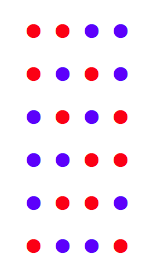
\includegraphics[width = 0.2\textwidth]{figures/marbles}
\end{center}

\[
{4 \choose 2} = \frac{4!}{2! \times 2!} = \frac{24}{2 \times 2} = 6.
\]

\end{frame}



%%%%%%%%%%%%%%%%%%%%%%%%%%%%%%%%%%%%%%%%%%
\begin{frame}

\disc{Example: how many handshakes take place between a group of 6 people if everyone need to shake hands with everyone else?}
Same questions: how many combinations of 2 numbers among $\{1, 2, 3, 4, 5, 6\}$ are there?
\uncover<2->{

\begin{center}
\{1,2\} \{1,3\} \{1,4\} \{1,5\} \{1,6\} \\
\{2,3\} \{2,4\} \{2,5\} \{2,6\}         \\
\{3,4\} \{3,5\} \{3,6\}                 \\
\{4,5\} \{4,6\}                         \\
\{5,6\}                                 \\
\end{center}
\[
{6 \choose 2} = \frac{6!}{4!2!} = \frac{6 \times 5}{2 \times 1} = 15
\]
}



\end{frame}

%%%%%%%%%%%%%%%%%%%%%%%%%%%%%%%%%%%%%%%%%%
\begin{frame}%\frametitle{}
Example: Poker hand. A standard poker deck has 52 cards, in four suits (clubs, diamonds, hearts, spades) of thirteen cards each (2, 3, ..., 10, Jack, Queen, King, Ace).
\disc{How many poker hands (5 cards) can be dealt from a deck of 52 cards?}
\pause
Combinations, choose 5 out of 52 different cards.
\[
{52 \choose 5} = \frac{52!}{47!5!} = \frac{52 \times 51 \times 50 \times 49 \times 48}{5 \times 4 \times 3 \times 2 \times 1} = 2,598,960
\]
\end{frame}



%%%%%%%%%%%%%%%%%%%%%%%%%%%%%%%%%%%%%%%%%%
\begin{frame}\frametitle{Properties of combinations ${n \choose r} = \frac{n!}{(n-r)!r!}$}

\begin{enumerate}
\item
\[{n \choose 1} = n ~~~~~~~~~~~~~~~~~~~~~~~~ {n \choose n} = 1~~~~~~~~~~~~ ~~~~~~~~~~~~\]
\pause
\item
\[{n \choose r} = {n \choose n - r} ~~~~~~~~~~~~~~~~~~~~~~~~~~~~~~~~~~~~~~~~~~~~~~~~~\]
\pause
\item
\[
{n \choose r} = {n-1 \choose r} + {n-1 \choose r-1}, \quad 1\leq r \leq n ~~~~~~~~~~~~~~~~~
\]
\end{enumerate}
\end{frame}

%%%%%%%%%%%%%%%%%%%%%%%%%%%%%%%%%%%%%%%%%%
\begin{frame}\frametitle{Binomial theorem}

\[
(a + b)^n = \sum_{k = 0}^n {n \choose k} a^k b^{n-k}
\]
{\it Proof: 1) mathematical induction or 2) combinatorial consideration.}\\
\pause
Think about license plates that are formed by $n$ digits, where each digit can be a letter or a number.
$a = 26, b = 10$. \\
\pause
Total number of distinct plates:
\[
N = (a + b)^n = N_0 + N_1 + \cdots + N_n,
\]
where $N_k$ is the number of distinct plates that contains exactly $k$ number of letters.
\pause
\[
N_k = {n \choose k} \times a^k \times b^{n-k}
\]
\vfill
%\Note{By definition, $0! = 1$}
\end{frame}




%%%%%%%%%%%%%%%%%%%%%%%%%%%%%%%%%%%%%%%%%%
\section{Multinomial coefficients}
%%%%%%%%%%%%%%%%%%%%%%%%%%%%%%%%%%%%%%%%%%
\begin{frame}\frametitle{Multinomial coefficients}
\disc{
Example: a police department of 10 officers wants to have 5 of the officers patrol streets, 2 doing paperwork, and 3 at the donut shop, how many
ways can this be done?}

\uncover<2->{
\[
{10 \choose 5}{5 \choose 2}{3 \choose 3} = \frac{10!}{5! (10-5)!}\cdot \frac{5!}{3! (5-3)!} = \frac{10!}{5!3! 2!}
\]
}

\uncover<3->{
\begin{dinglist}{\DingListSymbolA}
\item  \hl{Multinomial coefficient}: a set of $n$ distinct items is to be
divided into $r$ distinct groups of respective sizes $n_1, \ldots, n_r$, where $n_1 + n_2 + \cdots + n_r = n$.
Number of possible divisions is
\[
{n \choose n_1, n_2, \ldots, n_r} \stackrel{\text{def}}{=} \frac{n!}{n_1!n_2! \cdots n_r!}
\]
\end{dinglist}


}
\end{frame}

%%%%%%%%%%%%%%%%%%%%%%%%%%%%%%%%%%%%%%%%%%
\begin{frame}%\frametitle{Multinomial Theorem}

\begin{itemize}
\item
\[
{n \choose n_1, n_2, \ldots, n_r} = {n \choose n_1}{n-n_1 \choose n_2}{n-n_1-n_2 \choose n_3}\cdots{n_r \choose n_r}
\]
\pause

\item When $r = 2$, becomes binomial coefficient (choose function)
\[
{n \choose n_1, n_2} = {n \choose n_1}
\]
Note that $n_1 + n_2 = n$

\pause
\item Multinomial Theorem
\[
(a_1 + a_2 + \cdots + a_r)^n = \sum_{n_1 + \cdots + n_r = n} {n \choose n_1, n_2, \ldots, n_r} a_1^{n_1} a_2^{n_2} \cdots a_r^{n_r}
\]

\pause
\item The Binomial theorem is a special case when $r = 2$.
\end{itemize}

\end{frame}

%%%%%%%%%%%%%%%%%%%%%%%%%%%%%%%%%%%%%%%%%%






\end{document}
